
\documentclass[journal]{IEEEtran}
\usepackage{blindtext}
\usepackage{graphicx}
\usepackage{filecontents}
\usepackage{natbib}
\usepackage{bibentry}
\usepackage{booktabs,chemformula}

\usepackage{lipsum}
\usepackage{multirow, tabularx, caption, booktabs}
\usepackage{makecell}
\renewcommand\cellalign{rc}
\usepackage{siunitx}
\usepackage{listings}
\sisetup{table-format=1.1}
\usepackage{color}

\definecolor{codegreen}{rgb}{0,0.6,0}
\definecolor{codegray}{rgb}{0.5,0.5,0.5}
\definecolor{codepurple}{rgb}{0.58,0,0.82}
\definecolor{backcolour}{rgb}{0.95,0.95,0.92}

\lstdefinestyle{mystyle}{
	backgroundcolor=\color{backcolour},   
	commentstyle=\color{codegreen},
	keywordstyle=\color{magenta},
	numberstyle=\tiny\color{codegray},
	stringstyle=\color{codepurple},
	basicstyle=\footnotesize,
	breakatwhitespace=false,         
	breaklines=true,                 
	captionpos=b,                    
	keepspaces=true,                 
	numbers=left,                    
	numbersep=5pt,                  
	showspaces=false,                
	showstringspaces=false,
	showtabs=false,                  
	tabsize=2
}

\lstset{style=mystyle}


\usepackage{listings}

% Some very useful LaTeX packages include:
% (uncomment the ones you want to load)


% *** MISC UTILITY PACKAGES ***
%
%\usepackage{ifpdf}
% Heiko Oberdiek's ifpdf.sty is very useful if you need conditional
% compilation based on whether the output is pdf or dvi.
% usage:
% \ifpdf
%   % pdf code
% \else
%   % dvi code
% \fi
% The latest version of ifpdf.sty can be obtained from:
% http://www.ctan.org/tex-archive/macros/latex/contrib/oberdiek/
% Also, note that IEEEtran.cls V1.7 and later provides a builtin
% \ifCLASSINFOpdf conditional that works the same way.
% When switching from latex to pdflatex and vice-versa, the compiler may
% have to be run twice to clear warning/error messages.






% *** CITATION PACKAGES ***
%
%\usepackage{cite}
% cite.sty was written by Donald Arseneau
% V1.6 and later of IEEEtran pre-defines the format of the cite.sty package
% \cite{} output to follow that of IEEE. Loading the cite package will
% result in citation numbers being automatically sorted and properly
% "compressed/ranged". e.g., [1], [9], [2], [7], [5], [6] without using
% cite.sty will become [1], [2], [5]--[7], [9] using cite.sty. cite.sty's
% \cite will automatically add leading space, if needed. Use cite.sty's
% noadjust option (cite.sty V3.8 and later) if you want to turn this off.
% cite.sty is already installed on most LaTeX systems. Be sure and use
% version 4.0 (2003-05-27) and later if using hyperref.sty. cite.sty does
% not currently provide for hyperlinked citations.
% The latest version can be obtained at:
% http://www.ctan.org/tex-archive/macros/latex/contrib/cite/
% The documentation is contained in the cite.sty file itself.






% *** GRAPHICS RELATED PACKAGES ***
%
\ifCLASSINFOpdf
  % \usepackage[pdftex]{graphicx}
  % declare the path(s) where your graphic files are
  % \graphicspath{{../pdf/}{../jpeg/}}
  % and their extensions so you won't have to specify these with
  % every instance of \includegraphics
  % \DeclareGraphicsExtensions{.pdf,.jpeg,.png}
\else
  % or other class option (dvipsone, dvipdf, if not using dvips). graphicx
  % will default to the driver specified in the system graphics.cfg if no
  % driver is specified.
  % \usepackage[dvips]{graphicx}
  % declare the path(s) where your graphic files are
  % \graphicspath{{../eps/}}
  % and their extensions so you won't have to specify these with
  % every instance of \includegraphics
  % \DeclareGraphicsExtensions{.eps}
\fi
% graphicx was written by David Carlisle and Sebastian Rahtz. It is


% correct bad hyphenation here
\hyphenation{op-tical net-works semi-conduc-tor}


\begin{document}
%
% paper title
% can use linebreaks \\ within to get better formatting as desired
\title{Multiclass classification of songs' genre using one-vs-all and multinomial logistic regression}

\author{Anonymous}

% make the title area
\maketitle


\begin{abstract}
%\boldmath
The data analysis project, in the scope of Machine Learning Basic Principles course, focuses on multiclass classification to identify song genre using a custom subset of the Million Song Dataset [1], and the labels obtained from AllMusic.com [Give Ref]. Over the course of the project, 3 different methods were used to optimize and improve the accuracy of the song identification, namely, 'K Nearest Neighbours (KNN) with Low Dimensional Embedding', 'Multinomial Logistic Regression' and 'One vs All (OvA) Logistic Regression'. The initial method 'KNN with LDE' employs Principal Component Analysis [insert reference] to extract useful features out of the high-dimensional dataset and then uses KNN algorithm to create target clusters. On the other hand, Multinomial and OvA methods use probablistic models to classify target classes where the main difference occurs in the modeling assumptions behind each of the two models. The KNN with LDE approach was not able to breach the accuracy threshold, whereas OVA and MLR were both able to do so satisfactorily.
\blindtext[1]
\end{abstract}
% IEEEtran.cls defaults to using nonbold math in the Abstract.
% This preserves the distinction between vectors and scalars. However,
% if the journal you are submitting to favors bold math in the abstract,
% then you can use LaTeX's standard command \boldmath at the very start
% of the abstract to achieve this. Many IEEE journals frown on math
% in the abstract anyway.

% Note that keywords are not normally used for peerreview papers.
\begin{IEEEkeywords}
IEEEtran, journal, \LaTeX, paper, template.
\end{IEEEkeywords}






% For peer review papers, you can put extra information on the cover
% page as needed:
% \ifCLASSOPTIONpeerreview
% \begin{center} \bfseries EDICS Category: 3-BBND \end{center}
% \fi
%
% For peerreview papers, this IEEEtran command inserts a page break and
% creates the second title. It will be ignored for other modes.
\IEEEpeerreviewmaketitle



\section{Introduction}
Music, by no doubt, has become an imperative part of people's life. People prefer listening to their favorite genre of songs for more personalized experience. Because of the availability of tons of songs, listeners crave for more personalized experience while at the same time, they prefer non-static music for mood augmentation. \par
The project, in particular focuses on finding a pattern to identify the genre of songs. The identification pattern can help to build an online recommendation platform using exisiting databse of users so that listeners can have more customized experience while in search for new songs. During the entire project, we address the question that given a list of songs, how well can we analyze the audio to find a pattern that helps us identiy songs that belong to similar genre of music; which is to say that we construct a predictor h(x) for each genre (Y) using the features (x) of the songs and map it to a probability h(x). Simpler this tasks may seem for a certain type of songs (e.g. heavy metal vs classical), the classification problem can become difficult for other types (e.g.rock vs blues).

%\subsection{Subsection Heading Here}
%\blindtext

\section{Data Analysis}
The dataset used for the project is a custom subset of the Million Song Dataset [1], and the labels were obtained from AllMusic.com [give ref.]. For simplicity, each song has been assigned only one label that corresponds to the most representative genre. The 10 labels are :
\begin{enumerate}
	\item Pop Rock
	\item Electronic
	\item Rap
	\item Jazz
	\item Latin
	\item RnB
	\item International
	\item Country
	\item Reggae
	\item Blues
\end{enumerate}
\begin{figure}[h!]
The layout of a single example, representing one song, is as follows: \par
\begin{center}
	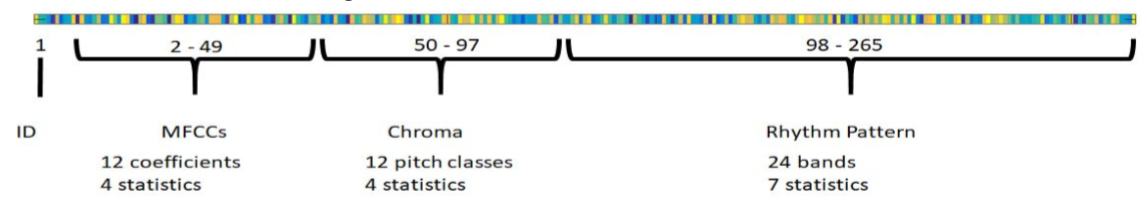
\includegraphics[width=200pt]{images/1_ExampleVectorStructure.PNG}
	\caption{Layout of Example Vector}
	\label{fig: Fig.1}
\end{center}
\end{figure}

\begin{figure}[h!]
The feature vector for each song thus consists of 12 coefficients representing MFFCs (using 4 statistics each), 12 pitch classes representing Chroma (using 4 statistics each), and 24 bands representing Rythm Patterns (using 7 statistics each). The details on the structure of each component of the example vector is as below: \par
\begin{center}
	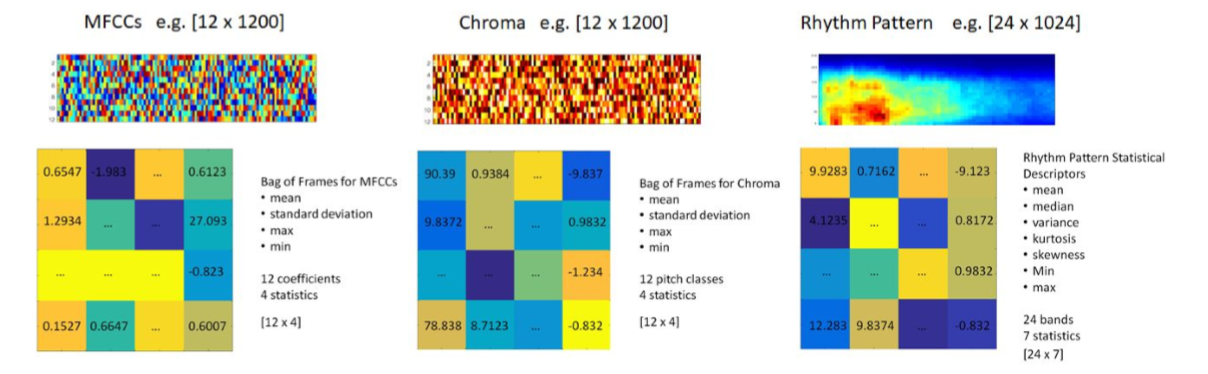
\includegraphics[width=200pt]{images/1_ExampleVectorStructure_2.PNG}
	\caption{Structural Representation of Example Vector}
	\label{fig:Fig.2}
\end{center}
\end{figure}

It was evident that the example features have high dimensionality, so it was decided to test an unsupervised learning approach to select create a lower dimensional dataset out of the existing dataset, to \textbf{potentially} improve performance and eliminate redundancy in the dataset. The approach adopted for this was \textbf{low dimensional embedding} [insert reference]. \par

\section{Methods and experiments}
Multiclass classification problem was explored using three different methods: \par
\begin{itemize}
	\item KNN clustering with low dimensional embedding
	\item Multinomial logistic regression
	\item One-vs-All (OvA)
\end{itemize}

\subsection{KNN clustering with low dimensional embedding}
Low dimensional embedding with KNN clustering approach was adopted first to see if it was at all possible to reduce the high dimensions, so that the performance and accuracy issues normally associated with them could be sidestepped.\par

This technique employs Principal Component Analysis [insert reference] to extract useful features out of the high-dimensional dataset, essentially projecting the features to a lower dimensional space, by retaining the top $n$ principal components which yield the highest explained variance. Next, it applies K-NN clustering on the low-dimensional dataset, with the prior PCA helping to prevent the ML algorithm from succumbing to the curse of dimensionality [insert reference]. \par

In our approach, we first reduced the dimensions of both our training and test datasets using PCA, followed by the application of the K-NN algorithm to acquire a model that fits our samples to appropriate labels. This model was then applied to the training and test sets, and the accuracy for both applications measured. \par

The approach was repeated for different values for dimensionality reduction and $K$ nearest neighbors, with the maximum accuracy finally being found at $K = 22$ and $n = 21$. The final accuracy results were less than satisfactory, although it was evident that the classification task was greatly expedited because of the reduced complexity of the lower dimensional dataset. \par

\textit{Due to the dissatisfactory results, it was decided to not pursue a dimensional reduction approach any further; we switched to the employment of Logistic Regression algorithms for solving the problem.} \par

\subsection{Difference between multinomial logistic regression and One-vs-All (OVA) classification}
Before delving into the two logistic regression techniques, let's try to understand the difference between both. The main difference occurs in the modeling assumptions behind each of the two models. Let's assume that there are K classes. For OVA, the assumption is that there are K independent classification problems, one for each class, i.e., for class i, we learn a logistic (probability) model of the form $\dfrac{1}{1+exp(-\beta_{i}^Tx)}$ and each of these K problems are independent of the other K-1 logistic regression problems. Whereas for Multinomial model, we assume that there is a multinomial conditional distribution,  such that for a class i we have the following logistic model $\dfrac{exp(-\beta_{i}^Tx)}{\sum_{j=1}^{K}exp(-\beta_{j}^Tx)}$. As can be seen immediately, learning $\beta_i$ for a particular class i immediately affects the model for other classes j through the joint model.\\

\subsection{Multinomial logistic regression}
Multinomial Logistic Regression is the linear regression analysis technique used when the dependent variable is nominal with more than two levels. Thus it is an extension of logistic regression, which analyzes dichotomous (binary) dependents. One of the major reasons for choosing multinomial logistic regression is because it works well on big data irrespective of different areas. \par
For the data analysis project, same technique was used like the logistic regression for binary classification until calculating the probabilities for each target. Once the probabilities were calculated, these were transferred into one hot encoding and cross entropy method was used for calculating the properly optimized weights. The idea is to construct a linear predictor function that constructs a score from a set of weights that are linearly combined with the features of a given observation using a dot product: \par
\begin{equation}
	score(X_i,k) = \beta_k . X_i,
\end{equation}
where $X_i$ (in our case) is the vector that contains the training data of songs, $\beta_k$ is a vector of weights (or regression coefficients) corresponding to k=10 outcomes of songs' genre, and $score(X_i, k)$ is the score associated with assigning each observation i to category k. \par
The following inforgraph explains the idea very well \par
\begin{center}
	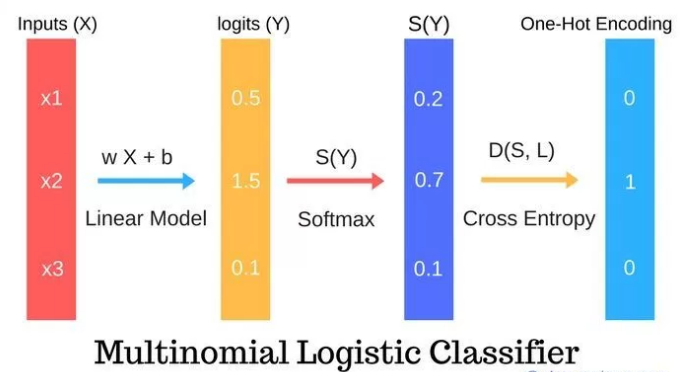
\includegraphics[width=\columnwidth]{images/how_it_works.png}
\end{center}

Just like we have sigmoid function in binary logistic regresssion, softmax function does the job in multinomial logistic regression. The Softmax function is a probabilistic function which calculates the probabilities for the given score and returns the high probability value for the high scores and fewer probabilities for the remaining scores. Therefore, each observation i in the training dataset (X) was evaluated on k=10 predictors (h(x)) and then, softmax function was used to find the highest probabilitic class to which the observation i belongs. \par
The last step used in the multinomial logistic regression is the cross-entropy. It is a distance calculation function which takes the calculated probabilities from softmax function and then creates one-hot-encoding matrix to calculate the distance. For the right target class, the distance value is less, and the distance values are larger for the wrong target class. \par
%\subsection{Challenges with Multinomial Logistic Regression}
The major challenge faced with this particular technique was to get the logitic loss to converge. Different number of iterations and different implementations of multinomial logistic regression were used. $sklearn.linear-model.LogisticRegression$ [2] function from Python's scikit-learn library was also experimented with different number of iterations (upto 1000 which takes around 5 to 10 minutes), and different solvers like ‘newton-cg’, ‘lbfgs’, ‘sag’, ‘saga’. The best result was obtained using 'newton-cg' solver. 

\subsection{One vs All (OvA)}
The second approach explored for this project was One-vs-All (also called One-vs-Rest) Classification. We train one classifier for every class, taking the samples for that particular class as positive, while the remaining samples are treated as negative. \par
The base classifer must yield a real-valued confidence score for the decision, as opposed to merely a class label, since discrete class labels could become ambiguous if results from multiple classifiers yield different labels for the same sample. \par

An algorithm describing the procedure is as follows:
\begin{itemize}
\item\textit{Inputs to the algorithm:}
\begin{itemize}
\item dataset of samples $X$ and labels $y$, where $y_{i} \in \{1, 2, ..., N\}$ is the label for the particular sample $X_{i}$
\item $L$, a binary classification training algorithm 
\end{itemize}
\item\textit{Outputs of the algorithm:}
\begin{itemize}
\item a set of classifiers $c_{n}$ for $n \in \{1, 2, ..., N\}$
\end{itemize}
\item\textit{Mechanism:}
\begin{itemize}
\item For every $n \in \{1, 2, ..., N\}$
	\begin{itemize}
	\item Build a separate label vector $z$, with $z_{i} = 1$ if $y_{i} = n$ and $z_{i} = 0$ for all other $y_{i}$
	\item Apply training algorithm $L$ on samples $X$ and label vector $z$, to get $c_{n}$ 
	\end{itemize}
\end{itemize}
\end{itemize}\par
Concretely deciding which class an unseen sample $x$ belongs to requires the application of all the obtained classifiers $c_{n}$ to it, and then choosing the label $n$ whose classifier yields the largest confidence score:
\begin{center}
${\hat{y}} =\underset{n\in\{1, 2, ..., N\}}{argmax} c_{n}(x)$
\end{center} \par
Two potential issues with the OVR are approach are:
\begin{itemize}
\item The confidence values can be different in terms of scale between each binary classifier
\item Despite the training set having a balanced class distribution, the binary classifiers will see it as unbalanced since the number of negative labels will (most likely) be much greater than the number of positive labels.
\end{itemize}
In this project's implementation of the OVR approach, the logistic regression algorithm was used to generate $N$ separate classifiers. The final label for each was decided based on the classifier that results in the best confidence score. Different number of iterations and different implementations of multinomial logistic regression were used. $sklearn.linear-model.LogisticRegression$ [2] function from Python's scikit-learn library was also experimented with different number of iterations (upto 1000 which takes around 5 to 10 minutes), and different solvers like ‘newton-cg’, ‘lbfgs’, ‘sag’, ‘saga’. The best result was obtained using 'newton-cg' solver. 

\section{Results}
Table-1 indicates the results for accuracy while table 2 indicates results for LogLoss.Among the many attempts that were made, results for the few are summarized below: \par
\begin{table}[!htb]
	\captionsetup{size=footnotesize}
	\caption{\textbf{Accuracy}} \label{tab:freq}
	\setlength\tabcolsep{0pt} % let LaTeX compute intercolumn whitespace
	\footnotesize\centering
	%This table provides the frequencies.
	
	\smallskip 
	\begin{tabular*}{\columnwidth}{@{\extracolsep{\fill}}rcccr}
		\toprule
		Attempt  & Method & Training Accuracy & Validation Accuracy & Kaggle Result \\
		\midrule
		1   & LDE with KNN & 57.04\%   & 53.03\%    & \% \\
		2   & Multinomial   & 74.53\%    & 63.14\%     & 62.13\% \\
		3   & Multinomial   & 75.8\%     & 63.90\%     & 62.483\% \\
		4   & OvR   & 75.9\%     & 63.5\%     & 62.88\% \\
		\midrule
		Best & OvR & 75.9\%     & 63.5\%     & 62.88\% \\
		\bottomrule
	\end{tabular*}
\end{table}

\begin{table}[!htb]
	\captionsetup{size=footnotesize}
	\caption{\textbf{LogLoss}} \label{tab:freq}
	\setlength\tabcolsep{0pt} % let LaTeX compute intercolumn whitespace
	\footnotesize\centering
	%This table provides the frequencies.
	
	\smallskip 
	\begin{tabular*}{\columnwidth}{@{\extracolsep{\fill}}rcccr}
		\toprule
		Attempt  & Method & Training\verb!_!Accuracy & Validation\verb!_!Accuracy & Kaggle\verb!_!Result \\
		\midrule
		1   & Multinomial   & 75.8\%    & 63.90\%   & 2.60627 \\
		2   & OvR   & 75.8\%     & 63.90\%     & 3.07390 \\
		\midrule
		Best   & Multinomial   & 75.8\%    & 63.90\%   & 2.60627 \\
		\bottomrule
	\end{tabular*}
\end{table}

\section{Conclusion}
In this project, various techniques were explored to obtain a Machine Learning model that scales to a moderately large dataset with high dimensionality. The K Nearest Neighbours with Low Dimensional Embedding approach was tested first, to see if any gains could be made by reducing the dataset to a lower dimensional space that was most representative of the variation inside the dataset. The technique yielded results that were counter-intuitive, which indicated that the majority of dimensions present inside the dataset did contain useful information that got lost with the reduction. After this deduction, we switched to logistic regression on the entire dataset, as it was. First, Multinomial Logistic Regression was applied, which yielded much improved accuracy and log-loss results. Furthermore, an OVA classification approach with logistic regression learner was also implemented, yielding comparable results to the MLR approach. In our experiments, OVA yielded marginally better results for the accuracy metric, whereas MLR yielded better results for the log-loss metric. \par




\blindtext


\ifCLASSOPTIONcaptionsoff
\newpage
\fi


\begin{thebibliography}{1}
	\bibitem{Million_Songs}	
	title  = "Million Song Dataset | scaling MIR research",
	url    = "https://labrosa.ee.columbia.edu/millionsong/",
	\bibitem{sklearn}
	title  = "sklearn.linearmodel.LogisticRegression",
	url    = "http://scikit-learn.org/stable/modules/generated/sklearn.linearmodel.LogisticRegression.html",
	\bibitem{PCA_definiation}
	title = ''Using PCA for Dimensionality Reduction''
	url = ''https://www.analyticsvidhya.com/blog/2015/07/dimension-reduction-methods/ ''
	\bibitem{Low dimensional embedding}
	title = ''Structure preserving embedding''
	author = ''Shaw, B.; Jebara, T.''
	year = ``2009''
	url = ``http://www.cs.columbia.edu/~jebara/papers/spe-icml09.pdf''
	\bibitem{Curse of Dimensionality}
	title = ``scikit-learn: Clustering and the curse of dimensionality''
	url = ``http://www.markhneedham.com/blog/2016/08/27/scikit-learn-clustering-and-the-curse-of-dimensionality/''
	
\end{thebibliography}

\newpage

\section{Appendices}
Important functions related to the project and source code is given below. Please feel free to comment for any improvement.
\begin{lstlisting}[language=Python, caption= KNN Clustering with Low Dimensional Embedding]
def KNN_with_LDE():
    """ Load Raw Data """
    print("loading data ...")
    # Load the Training Data
    data_path_x = "train_data.csv";
    songs_data = pd.read_csv("train_data.csv", header=None);
    # Load the True Labels
    data_path_y = "train_labels.csv";
    songs_labels = pd.read_csv("train_labels.csv", header=None);
    data_path_z = "test_data.csv";
    val_x = pd.read_csv("test_data.csv", header=None);

    """ Pre Process Data """
    print("preprocessing data ...")
    scaler = preprocessing.StandardScaler().fit(songs_data)
    scaler
    scaler.mean_
    scaler.scale_
    scaler.transform(songs_data)
    scaler.transform(val_x)

    """ Split training data into training data and test data for cross validation """
    print("partitioning data ...")
    train_x, test_x, train_y, test_y = train_test_split(songs_data, songs_labels, train_size=0.8, random_state=0);

    """ Perform feature reduction"""
    print("performing feature reduction ...")
    train_x_pca = PCA(21)
    train_x_pca.fit(train_x)
    train_x_reduced = train_x_pca.transform(train_x)
    test_x_reduced = train_x_pca.transform(test_x)
    val_x_reduced = train_x_pca.transform(val_x)

    """ Build the KNN model"""
    print("building model...")
    n_neighbors = 22
    we\section{Conclusion}
In this project, various techniques were explored to obtain a Machine Learning model that scales to a moderately large dataset with high dimensionality. The K Nearest Neighbours with Low Dimensional Embedding approach was tested first, to see if any gains could be made by reducing the dataset to a lower dimensional space that was most representative of the variation inside the dataset. The technique yielded results that were counter-intuitive, which indicated that the majority of dimensions present inside the dataset did contain useful information that got lost with the reduction. After this deduction, we switched to logistic regression on the entire dataset, as it was. First, Multinomial Logistic Regression was applied, which yielded much improved accuracy and log-loss results. Furthermore, an OVA classification approach with logistic regression learner was also implemented, yielding comparable results to the MLR approach. In our experiments, OVA yielded marginally better results for the accuracy metric, whereas MLR yielded better results for the log-loss metric. \parights = 'uniform'
    clf = neighbors.KNeighborsClassifier(n_neighbors, weights)
    clf.fit(train_x_reduced, np.asarray(train_y).ravel())

    """ Output accuracy results for Train and Test partitions"""
    print("Train Accuracy :: ", metrics.accuracy_score(train_y, clf.predict(train_x_reduced)));
    print("Test Accuracy ::  ", metrics.accuracy_score(test_y, clf.predict(test_x_reduced)));

	""" Predict the Test (unlabeled) Data """
	test_data_results = mul_lr.predict(val_x_reduced);
	""" Export the Test Data File """
	df = pd.DataFrame(test_data_results);
	df.to_csv('test_data_results.csv', index=False, header=False);
\end{lstlisting}

\begin{lstlisting}[language=Python, caption= Logistic Gradient Descent]
""" logistic_gradient_descent returns w_{opt}"""
def logistic_gradient_descent(x_vec,y_vec,N):

w = np.zeros((N,1));
w_opt = np.zeros((N,1));
a = 1e-5; """ Learning Rate """
yT = np.transpose(y_vec);
xT = np.transpose(x_vec);
error_margin = 0.0001;
e = 1e20;
_iter = 0;
min_error = e;
#for _iter in range(1000):
while(abs(e) > error_margin):
if (_iter > 1000):
break;
_num = math.exp(-np.dot(yT,np.dot(x_vec,w)));
_den = 1 + math.exp(-np.dot(yT,np.dot(x_vec,w)));
grad_w = -(5/N)*(_num/_den)*np.dot(xT,y_vec);
w = w - a*grad_w;
""" Computer Error """
e = math.log(1 + math.exp(-np.dot(yT,
			np.dot(x_vec,w))));

if (min_error > e):
min_error = e;
w_opt = w;
print (e);
_iter = _iter + 1;
#print (w.shape);
return (w_opt);
\end{lstlisting}

\begin{lstlisting}[language=Python, caption = Multinomial LogisticRegression]
""" Performs Multinomial Logistic Regression """

def mult_nomial_logr():
""" Prepare the Data """
# Load the Training Data
data_path_x = "path/train_data.csv";
songs_data = pd.read_csv
			(data_path_x, header=None);
# Lad the True Labels.
data_path_y = "path/train_labels.csv";
songs_target = pd.read_csv
			(data_path_y, header=None);
data_path_z = "path/test_data.csv";
test_data = pd.read_csv
			(data_path_z, header=None);

""" Split Data into Training and Validation """
train_x, test_x, train_y, test_y = 
train_test_split(songs_data, songs_target, 
			train_size=0.7, random_state=0);

"""Train multinomial logistic regression model"""
mul_lr = linear_model.LogisticRegression(multi_class='multinomial', max_iter=500, solver='netwon-cg').fit(train_x, train_y);
print ("Multinomial Logistic regression Train Accuracy :: ", metrics.accuracy_score(train_y, mul_lr.predict(train_x)));
print ("Multinomial Logistic regression Test Accuracy ::  ", metrics.accuracy_score(test_y, mul_lr.predict(test_x)));

""" Predict the Test Data """
test_data_results = mul_lr.predict(test_data);
""" Export the Test Data File """
df = pd.DataFrame(test_data_results);
df.to_csv('test_data_results.csv', index=False, header=False);
\end{lstlisting}

\begin{lstlisting}[language=Python, caption = OvR LogisticRegression]
""" Performs OvR Logistic Regression """
def mult_nomial_logr():
""" Prepare the Data """
# Load the Training Data
data_path_x = "path/train_data.csv";
songs_data = pd.read_csv(data_path_x, header=None);
# Load the True Labels.
data_path_y = "path/train_labels.csv";
songs_target = pd.read_csv(data_path_y, header=None);
data_path_z = "path/test_data.csv";
test_data = pd.read_csv(data_path_z, header=None);

""" Split Data into Training and Validation """
train_x, test_x, train_y, test_y = train_test_split(songs_data, songs_target, train_size=0.7, random_state=0);

"""Train multinomial logistic regression model"""
mul_lr = linear_model.LogisticRegression(multi_class='ovr', max_iter=500, solver='netwon-cg').fit(train_x, train_y);
print ("OvR Logistic regression Train Accuracy :: ", metrics.accuracy_score(train_y, mul_lr.predict(train_x)));
print ("OvR Logistic regression Test Accuracy ::  ", metrics.accuracy_score(test_y, mul_lr.predict(test_x)));

""" Predict the Test Data """
test_data_results = mul_lr.predict(test_data);
""" Export the Test Data File """
df = pd.DataFrame(test_data_results);
df.to_csv('test_data_results.csv', index=False, header=False);
\end{lstlisting}




\end{document}